\documentclass{beamer}
\begin{document}

% Content
%------------------------------------------------------------------------------------

\begin{frame}[t,mybg=placeholder,mytitle=standard,mycolor=digiPH_stem,dark]
	\only<1->{\Huge{Ukuran letak} }
\end{frame}

\begin{frame}[t,mybg=placeholder,mytitle=standard,mycolor=digiPH_stem,dark]
	\frametitle{Macam-macam ukuran letak}
	\begin{itemize}
		\item<1-> Kuartil
		\item<2-> Desil
		\item<3-> Prosentil
	\end{itemize}
\end{frame}

\begin{frame}[t,mybg=bg1,mytitle=imageplus,light]
	\frametitle{Definisi}

	\only<1->{\boxes{digiPH_leaf}{digiPH_writer}{
			\textbf{Ukuran letak} adalah rangkaian ukuran yang didasarkan letak dari suatu distribusi data
		}}

	\only<2->{
		\boxes{digiPH_gray}{digiPH_writer}{\textrm{Kuartil} adalah ukuran letak yang membagi suatu distribusi menjadi 4 (empat) bagian yang sama}
	}
\end{frame}

\begin{frame}[t,mybg=bg2,mytitle=center,light]
	\frametitle{Cara perhitungan kuartil}

	\boxes{white}{digiPH_writer}{\only<1>{Untuk data yang \textbf{tidak dikelompokkan}

			Susun data diurutkan dari yang memiliki \textit{nilai terkecil}}

		\only<2->{{\centering Cari letak kuartil, dengan rumus:}}

		\only<3->{kuartil 1
			\includegraphics<3->[width=30mm]{k1}

			kuartil 2
			\includegraphics<4->[width=30mm]{k2}

			kuartil 3
			\includegraphics<5->[width=30mm]{k3}}}
\end{frame}

\begin{frame}[t,mybg=bg2,mytitle=center,light]
	\frametitle{Cara perhitungan kuartil}

	\only<1-5>{Untuk data yang tidak dikelompokkan}

	\only<2-5>{Contoh:
		Carilah nilai kuartil pada rangkaian data berikut ini:
		\begin{tabular}{ccccccc}
			2  &  4  &  3  &  3  &  6  &  5  &  7  \\
			\hline
		\end{tabular}}

	\only<3-5>{Langkah :}

	\only<4-5>{susunan data :
		\begin{tabular}{ccccccc}
			2  &  3  &  3  &  4  &  5  &  6  &  7  \\
			\hline
		\end{tabular}}

	\only<5>{Letak kuartil:
		\begin{columns}
			\begin{column}{0.5\textwidth}
				\begin{itemize}
					\item<6-> 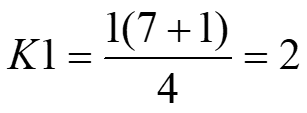
\includegraphics[width=25mm]{k4}
					\item<7-> 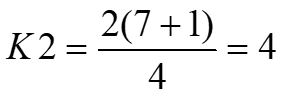
\includegraphics[width=25mm]{k5}
					\item<8-> 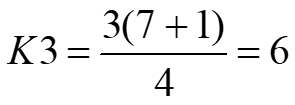
\includegraphics[width=25mm]{k6}
				\end{itemize}
			\end{column}
			\begin{column}{0.5\textwidth}
				\begin{itemize}
					\item<6-> terletak pada data yang ke-2(dua)
					\item<7-> terletak pada data yang ke-4(empat)
					\item<8-> terletak pada data yang ke-6(enam)
				\end{itemize}
			\end{column}
		\end{columns}}
	\only<6->{
		\centering Dengan demikian nilai K1 = 2,K2 = 4,K3 = 6
	}
\end{frame}

\begin{frame}[t,mybg=bg2,mytitle=standard,light]
	\frametitle{Cara perhitungan kuartil}

	\only<1->{Untuk data yang dikelompokkan}
	\only<2>{Susunan tabel
		\begin{center}
			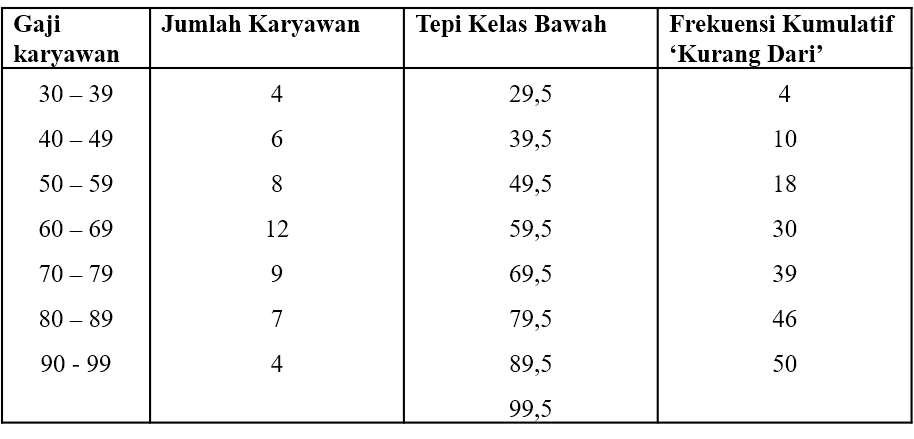
\includegraphics[width=100mm]{k21}
		\end{center}}

	\only<3->{Cari letak kuartil}

	\only<4->{Kuartil 1 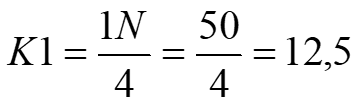
\includegraphics[width=30mm]{k31}

		kuartil 1 terletak pada data yang ke-12.5, yaitu pada kelompok ke-3 (tiga)}

	\only<5->{Kuartil 2 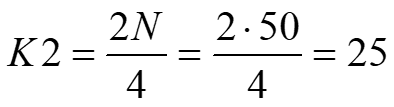
\includegraphics[width=30mm]{k32}

		kuartil 2 terletak pada data yang ke-25, yaitu pada kelompok ke-4 (empat)}

	\only<6->{Kuartil 3 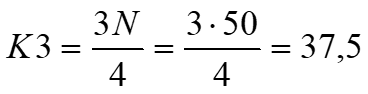
\includegraphics[width=30mm]{k33}

		kuartil 3 terletak pada data yang ke-37.5, yaitu pada kelompok ke-5 (lima)}
\end{frame}

\begin{frame}[t,mybg=placeholder,mytitle=standard,mycolor=digiPH_gray,light]
	\frametitle{Cara perhitungan kuartil}

	\only<1->{Untuk data yang dikelompokkan}


	\only<2-3>{Nilai Kuartil 1 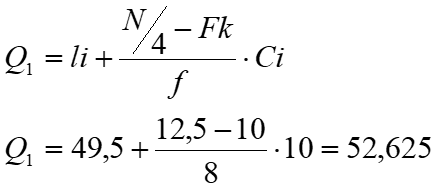
\includegraphics[width=45mm]{k41}}

	\only<4>{Nilai Kuartil 2 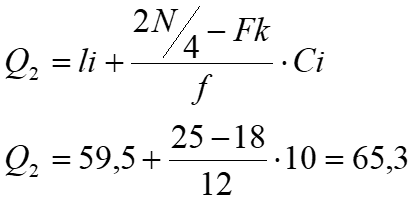
\includegraphics[width=45mm]{k42}}

	\only<5>{Nilai Kuartil 3 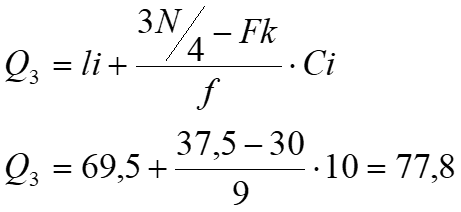
\includegraphics[width=45mm]{k43}}

	\only<3->{keterangan
		\begin{tabular}{cl}
			li  &  = Batas bawah letak kuartil  \\
			N   &  = Jumlah data  \\
			Fk  &  = Frekuensi kumulatif sebelum letak kuartil  \\
			f   &  = frekuensi pada letak kuartil  \\
			\hline
		\end{tabular}}
\end{frame}

\begin{frame}[t,mybg=bg1,mytitle=imageplus,light]
	\frametitle{Definisi}
	\boxes{digiPH_writer}{digiPH_gray}{
		\textmd{Desil} adalah ukuran letak yang membagi suatu distribusi data menjadi sepuluh (10) bagian sama besar.
	}
\end{frame}

\begin{frame}[t,mybg=bg1,mytitle=center,light]
	\frametitle{Cara perhitungan desil}

	\only<1>{Untuk data yang tidak dikelompokkan
		Susun data diurutkan dari yang memiliki \textit{nilai terkecil}}

	\only<2->{{\centering Cari letak desil, dengan rumus:}}

	\only<3->{
		Desil 1  \includegraphics<3->[width=30mm]{d1}

		Desil 5
		\includegraphics<4->[width=30mm]{d2}

		desil 9
		\includegraphics<5->[width=30mm]{d3}}


\end{frame}

\begin{frame}[t,mybg=bg2,mytitle=center,light]
	\frametitle{Cara perhitungan desil}

	\only<1-5>{Untuk data yang tidak dikelompokkan}

	\only<2-5>{Contoh:
		Carilah nilai desil pada rangkaian data berikut ini:
		\begin{tabular}{ccccccc}
			2  &  4  &  3  &  3  &  6  &  5  &  7  \\
			\hline
		\end{tabular}}

	\only<3-5>{Langkah :}

	\only<4-5>{susunan data :
		\begin{tabular}{ccccccc}
			2  &  3  &  3  &  4  &  5  &  6  &  7  \\
			\hline
		\end{tabular}}

	\only<5>{Letak desil
		\begin{columns}
			\begin{column}{0.5\textwidth}
				\begin{itemize}
					\item<6-> 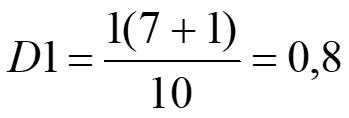
\includegraphics[width=25mm]{d4}
					\item<7-> 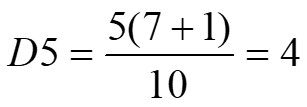
\includegraphics[width=25mm]{d5}
					\item<8-> 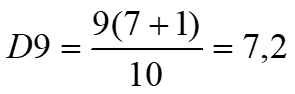
\includegraphics[width=25mm]{d6}
				\end{itemize}
			\end{column}
			\begin{column}{0.5\textwidth}
				\begin{itemize}
					\item<6-> terletak pada data yang ke-2(dua)
					\item<7-> terletak pada data yang ke-4(empat)
					\item<8-> terletak pada data yang ke-7(enam)
				\end{itemize}
			\end{column}
		\end{columns}}
	\only<6->{
		\centering Dengan demikian nilai D1 = 2,D5 = 4,D9 = 7
	}
\end{frame}

\begin{frame}[t,mybg=bg2,mytitle=standard,light]
	\frametitle{Cara perhitungan desil}

	\only<1->{Untuk data yang dikelompokkan}
	\only<2>{Susunan tabel
		\begin{center}
			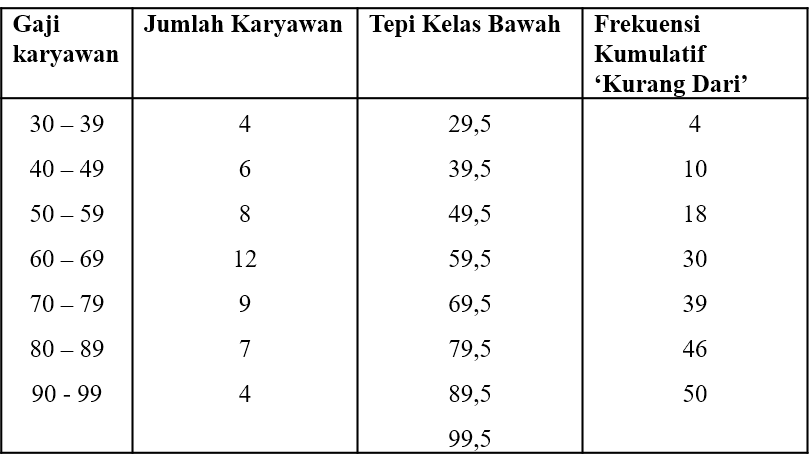
\includegraphics[width=100mm]{d21}
		\end{center}}

	\only<3->{Cari letak kuartil}

	\only<4->{Desil 1 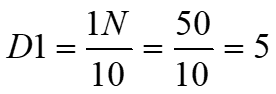
\includegraphics[width=28mm]{d31}

		desil 1 terletak pada data yang ke-5, yaitu pada kelompok ke-2 (dua)}

	\only<5->{Desil 5 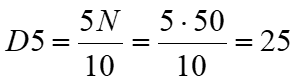
\includegraphics[width=28mm]{d32}

		desil 5 terletak pada data yang ke-25, yaitu pada kelompok ke-4 (empat)}

	\only<6->{Desil 9 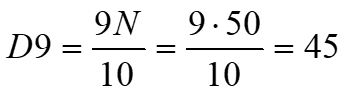
\includegraphics[width=28mm]{d33}

		desil 9 terletak pada data yang ke-45, yaitu pada kelompok ke-7 (tujuh)}
\end{frame}


\begin{frame}[t,mybg=bg3,mytitle=standard,light]
	\frametitle{Cara perhitungan desil}

	\only<1->{Untuk data yang dikelompokkan}


	\only<2-3>{Nilai Desil 1 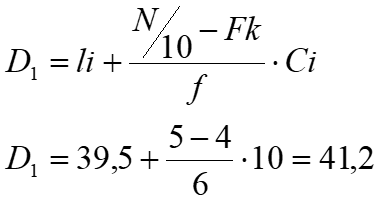
\includegraphics[width=45mm]{d41}}

	\only<4>{Nilai Desil 5 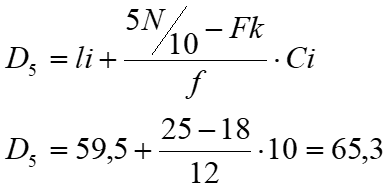
\includegraphics[width=45mm]{d42}}

	\only<5>{Nilai Desil 9 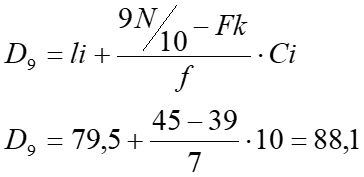
\includegraphics[width=45mm]{d43}}

	\only<3->{keterangan
		\begin{tabular}{cl}
			li  &  = Batas bawah letak kuartil  \\
			N   &  = Jumlah data  \\
			Fk  &  = Frekuensi kumulatif sebelum letak desil  \\
			f   &  = frekuensi pada letak desil  \\
			\hline
		\end{tabular}}
\end{frame}


\begin{frame}[t,mybg=bg1,mytitle=imageplus,light]
	\frametitle{Definisi}

	\only<1->{

		\boxes{digiPH_gray}{digiPH_writer}{Prosentil  adalah ukuran letak yang membagi suatu distribusi data menjadi seratus (100) bagian sama besar}
	}
\end{frame}


\end{document}
